\begin{chapter}{Referencial Teórico}
Este capítulo tem como objetivo apresentar o referencial teórico das ferramentas
mais importantes para o desenvolvimento do dispositivo proposto neste trabalho,
como i) piezoeletricidade; ii) operadores operacionais; iii) Conectores de
áudio; iv) ferramenta de desenvolvimento de placas de circuito impresso; v) captura de sinais
através da interface de áudio do computador; e, finalmente vi) ferramenta para a
emulação dos eventos de clique do \textit{mouse}.

\begin{section}{Piezoeletricidade}

Há certos elementos na natureza capazes de converter uma uma grandeza física em
outra. Por exemplo, transformar temperatura em tensão elétrica. Esses
elementos são chamados de transdutores~\cite{william}. Um grande exemplo de
transdutor é o microfone, que é capaz de converter o som, uma onda mecânica, em
sinais elétricos que são amplificados por um circuito e reproduzidos por algum
dispositivo de som, como alto-falantes. Muitas vezes transdutores são chamados
de sensores, porém esta denominação não é correta, pois, segundo~\cite{usher},
sensor é um dispositivo capaz de medir uma grandeza física, como é o caso do
termômetro que realiza a medição de temperatura. 

Há certos transdutores que são capazes de converter mais de uma grandeza física,
como é o caso do transdutor piezoelétrico. Esse transdutor utiliza a chamada
piezoeletricidade e é bastante utilizado em diversas aplicações diferentes. Seu
principio de funcionamento é dividido em efeito piezoelétrico direto e reverso
que serão brevemente descritos seguir.

\begin{subsection}{Efeito Piezoelétrico Direto}

O efeito piezoelétrico direto refere-se a capacidade de um material gerar tensão
elétrica quando submetido a estresses mecânicos como compressão ou
vibração~\cite{jaffe2012piezoelectric}. Muitos aparelhos eletrônicos utilizam
essa propriedade da piezoeletricidade. Por exemplo, piezos são bastantes
utilizados na indústria como uma ferramenta que ajuda a detectar a presença de
objetos em determinadas áreas. Quando há algum objeto sobre uma área desejada,
o peso desse objeto realiza uma força de compressão sobre o material
piezoelétrico produzindo uma tensão que pode ser medida por um sensor. Dessa
forma, uma máquina pode ``perceber'' que tem um objeto sobre a área desejada e
pode realizar a sua função pré-programada. É importante perceber que o piezo não
funciona como sensor, apenas converte uma grandeza física, nesse caso a força
peso causada pela massa do objeto, em uma energia capaz de ser medida por um
determinado instrumento.
  
\begin{figure}[!h]
	\centering
	\begin{minipage}[c]{\textwidth}
	\centering
	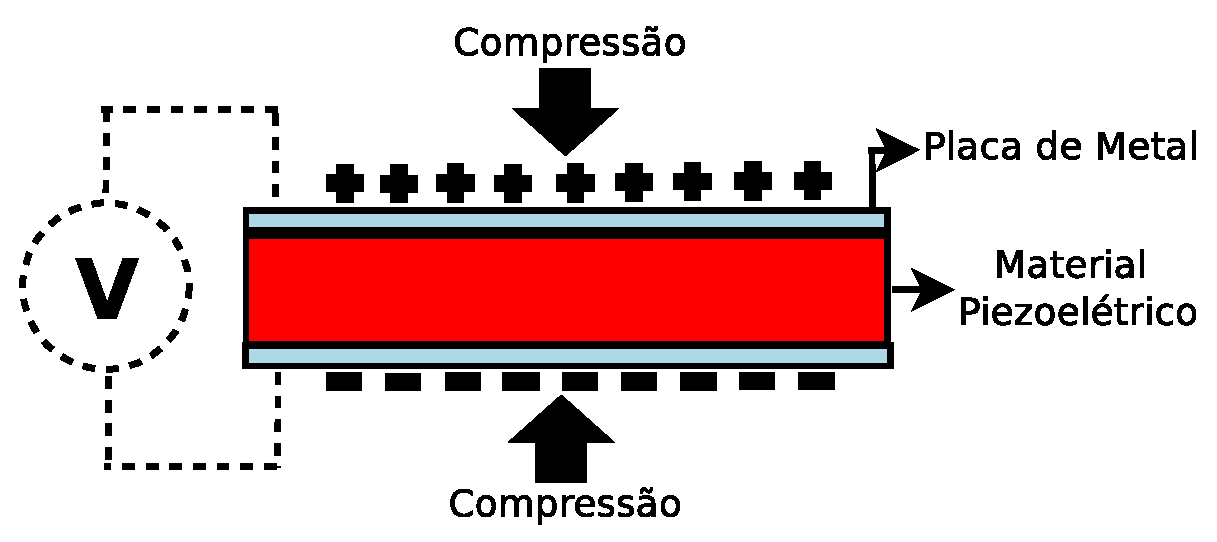
\includegraphics[width=0.9\linewidth]{fig/EfeitoPiezoEletricoDireto}
	\caption{Efeito piezoelétrico direto.}
	\label{fig:direto}
	\end{minipage}
\end{figure}

A Figura~\ref{fig:direto} mostra o princípio de funcionamento do efeito
piezoelétrico direto. Um material piezoelétrico --- um cristal de quartzo, por
exemplo --- é posicionado entre duas placas de metal. Para ocorrer a geração de
energia elétrica, é necessário algum tipo de estresse mecânico no material, como
compressão ou vibração. Quando as placas de metal são pressionadas, por exemplo,
ocorre uma diferença de potencial elétrico na superfície das placas como
consequência do chamado de efeito piezoelétrico direto.  É possível armazenar a
energia gerada pela compressão do material piezoelétrico e utilizá-la para
alimentar circuitos elétricos, substituindo as baterias por exemplo, como
realizado em~\cite{twitter}. 

\end{subsection}


\begin{subsection}{Efeito Piezoelétrico Reverso}
É possível realizar o processo contrário do efeito piezoelétrico direto. A
Figura~\ref{fig:reverso} ilustra o princípio de funcionamento do efeito
piezoelétrico reverso. Dado duas placas de metal separados por um material
piezoelétrico, é possível gerar perturbações mecânicas nessas placas. Para isso
é necessário aplicar um diferença de potencial elétrico nas placas que vibram
proporcionalmente a tensão aplicada~\cite{Lin12}. É possível gerar ondas de som a
partir das vibrações das placas de metal, mas para que isso ocorra as palcas
devem necessariamente vibrar em uma faixa de frequência entre 20~Hz e 20~Khz
(faixa de frequência audível ao ser humano).


\begin{figure}[!h]
	\centering
	\begin{minipage}[c]{\textwidth}
	\centering
	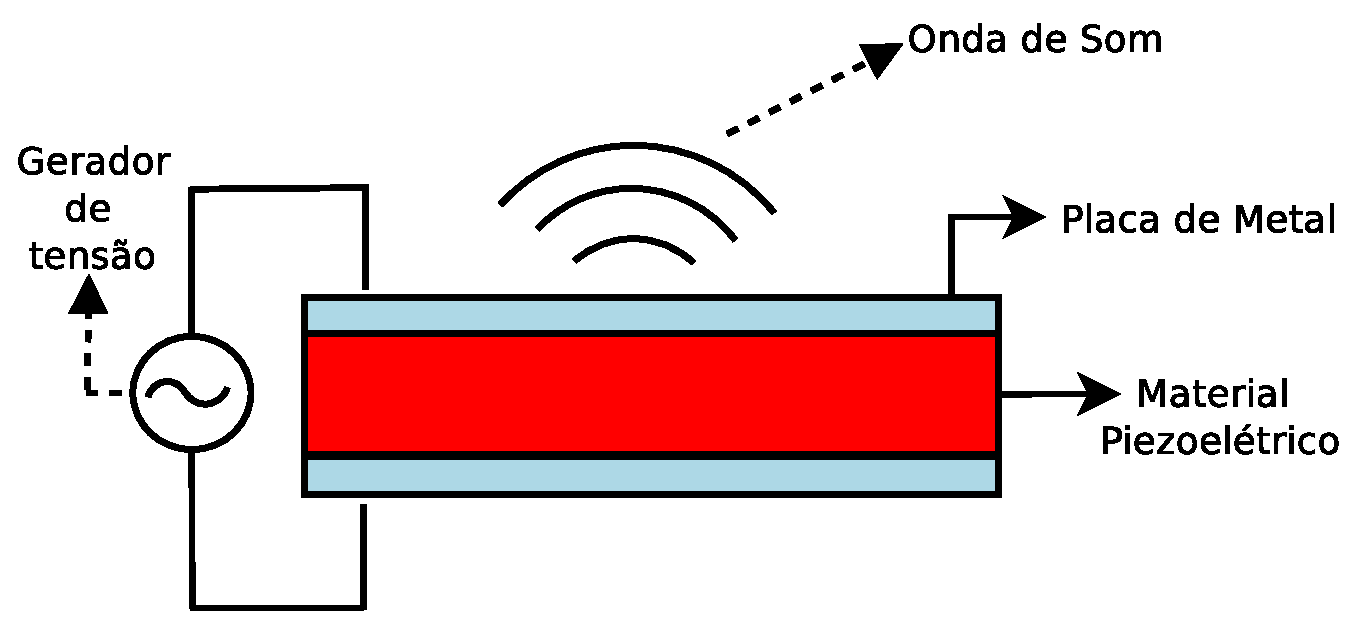
\includegraphics[width=0.9\linewidth]{fig/EfeitoPiezoEletricoReverso}
	\caption{Efeito piezoelétrico reverso.}
	\label{fig:reverso}
	\end{minipage}
\end{figure}

Muitos aparelhos eletrônicos utilizam o efeito piezoelétrico. Os sons de
sinalizações emitidos por computadores ao serem ligados ou quando há algum tipo
de problema no funcionamento no computador, são gerados por um dispositivo
chamado buzzer e é um bom exemplo de utilização do efeito piezoelétrico reverso.
Até mesmo alguns sonares utilizam o princípio desse fenômeno da
piezoeletricidade, onde é aplicado uma tensão modulada por PWM (do inglês,
\textit{pulse with modulation}) em um material piezoeletricidade que emite um
sinal ultrassom. Alguns desses instrumentos ultrassônicos são utilizados na área
médica para realização de cirurgias, como a maxilofacial onde é necessário
realizar cortes em tecidos ósseos~\cite{Carvalho17}.

\end{subsection}

\end{section}

\begin{section}{Amplificadores Operacionais}
O circuito eletrônico conhecido como amplificador operacional (opamp) é um componente
muito importante em cirtuitos elétricos que realiza operações especiais de
processamento de sinais~\cite{Richard2000}. A Figura~\ref{fig:opamp} mostra a
representação de um amplificador operacional.

\begin{figure}[!h]
	\centering
	\begin{minipage}[c]{\textwidth}
	\centering
	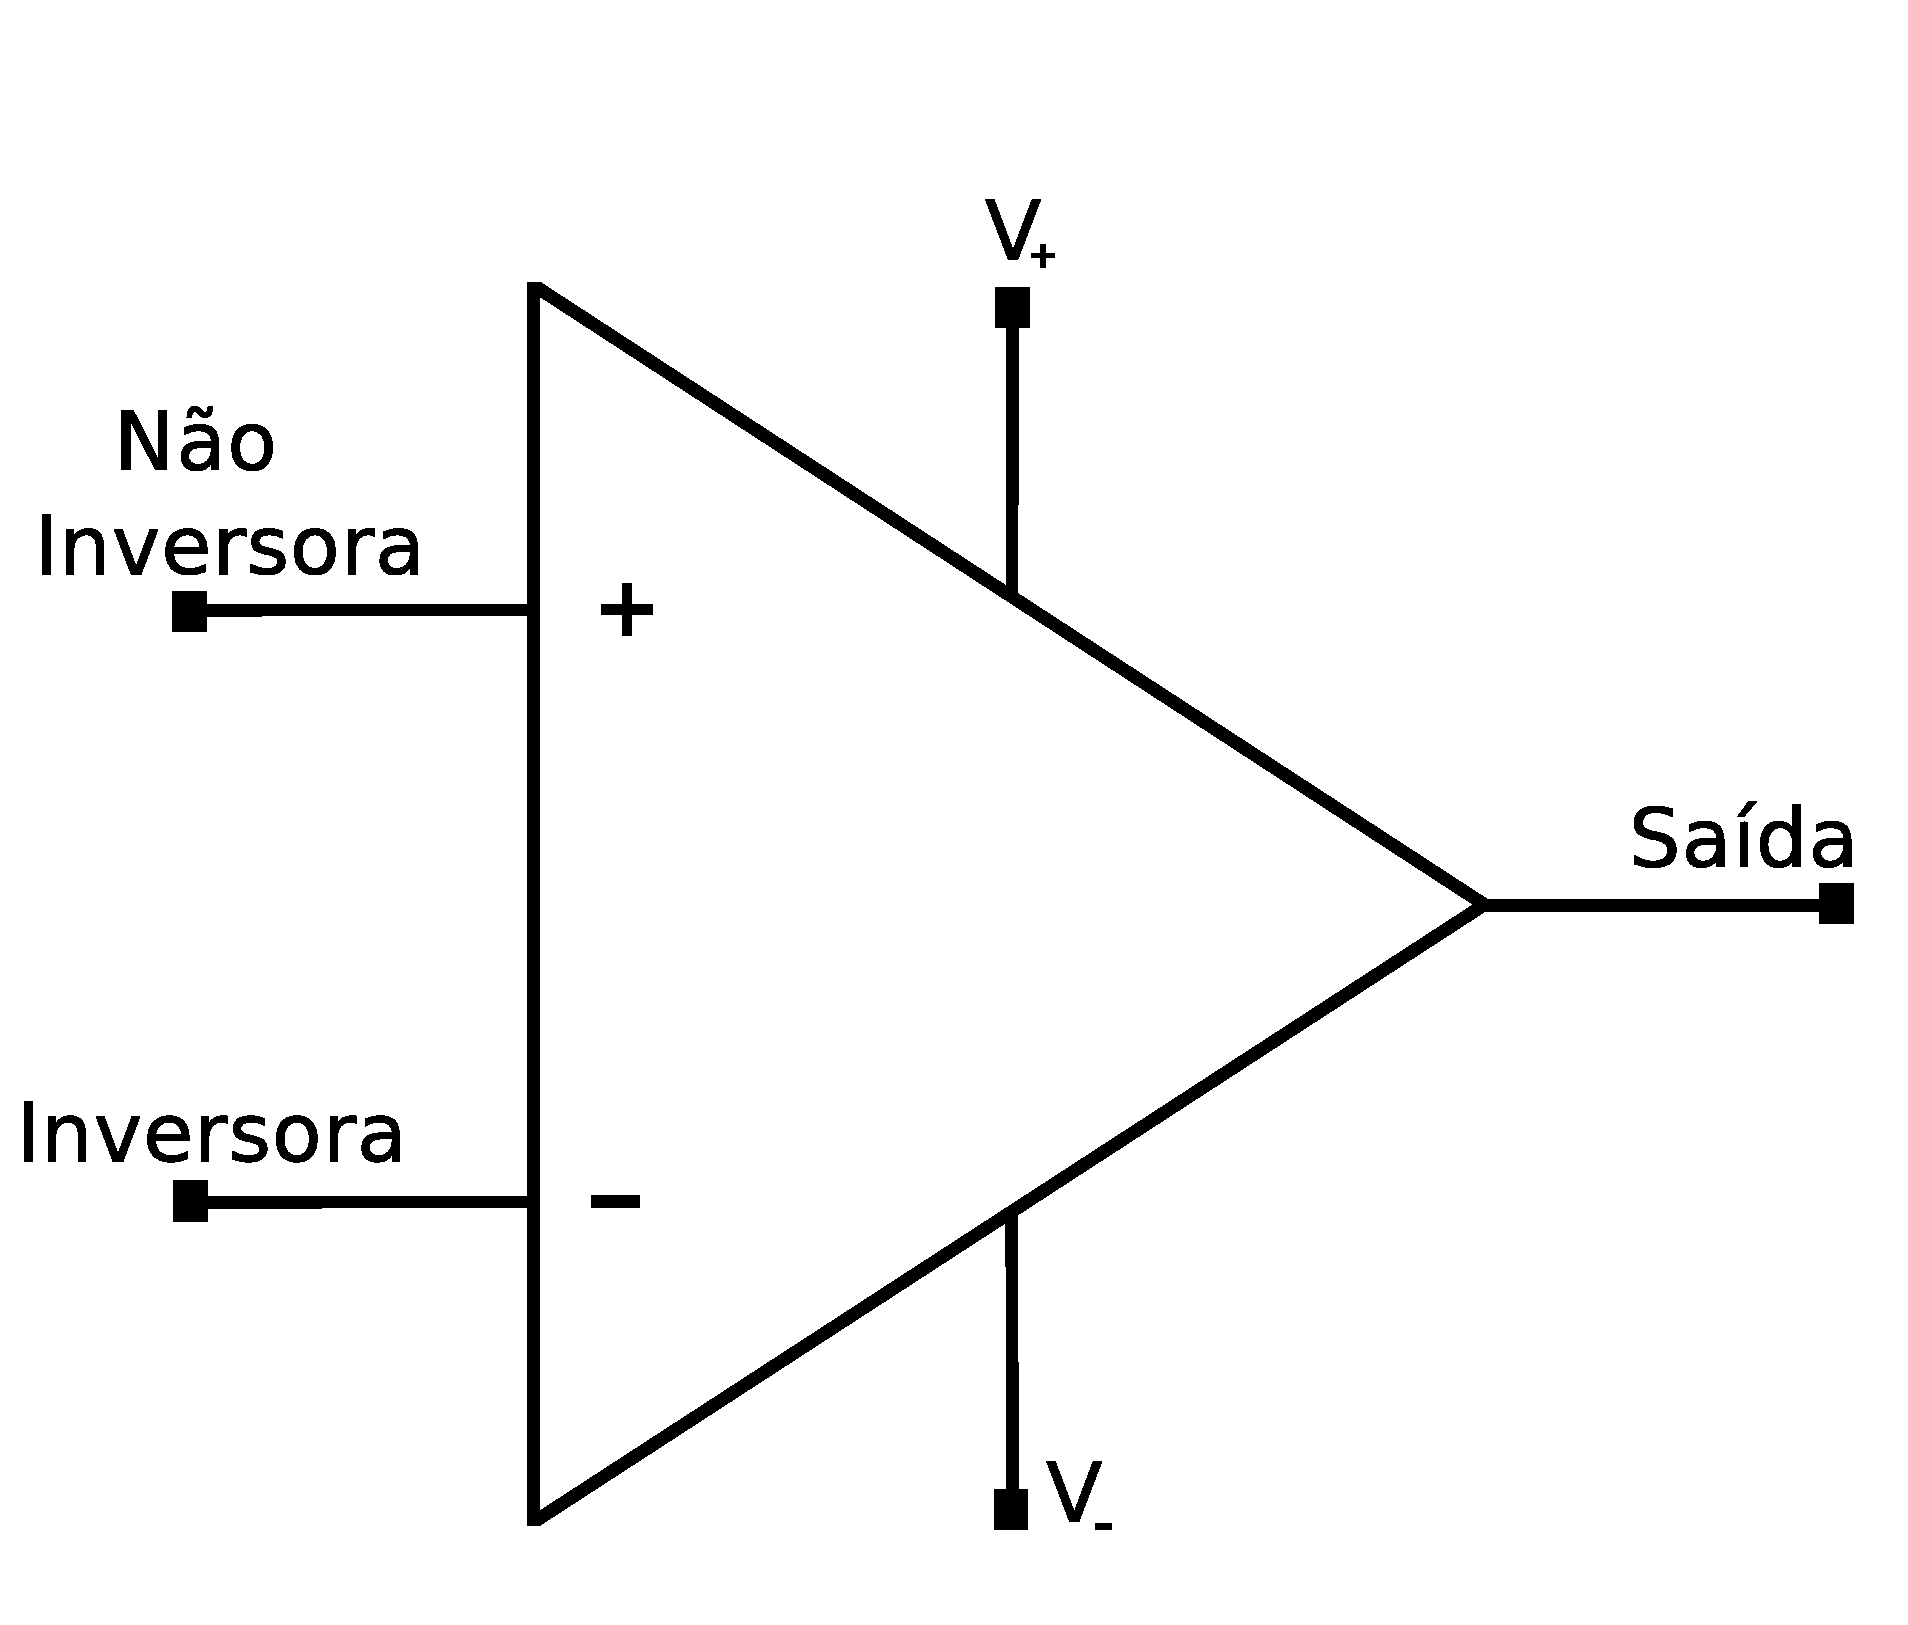
\includegraphics[width=0.5\linewidth]{fig/opamp}
	\caption{Representação de um amplificador operacional.}
	\label{fig:opamp}
	\end{minipage}
\end{figure}

O operador operacional ilustrado na Figura~\ref{fig:opamp} possui dois terminais
de alimentação, duas entradas --- inversora e não inversora --- e uma saída. A
entrada não inversora é convencionalmente representada pelo símbolo ``+'' e a 
entrada inversora é representada pelo símbolo ``-''. Quando é aplicado um sinal
na entrada não inversora, o sinal na saída possui a mesma fase do sinal de
entrada. Por outro lado, quando o sinal é aplicado na entrada inversora, o sinal
de saída possui uma fase contrária ao sinal de entrada. É importante ressaltar
que em alguns autores omitem a representação dos terminais de alimentação por
considerarem desnecessários e tenderem a sobrecarregar visualmente os esquemas
de circuitos, tornando-os mais difíceis de serem interpretados. Contudo fica
subentendido que os terminais de alimentação fazem parte do circuito, embora
muitas vezes não sejam mostrados.

A partir de várias combinações de resistores nos terminais do amplificador
operacional é possível executar funções muito úteis com os sinais de entrada, 
como multiplicação por um fator constante, soma, mudança de fase de sinal e
subtração~\cite{Nilson09}. Outro função bastante importante que pode ser
implementada com amplificadores operacionais é comparação de sinais. Dado dois
sinais, um em cada entrada, a saída é determinada a partir de uma comparação de
intensidade entre os dois sinais de entrada~\cite{Terrell96}.  
 

\begin{figure}[!h]
	\centering
	\begin{minipage}[c]{\textwidth}
	\centering
	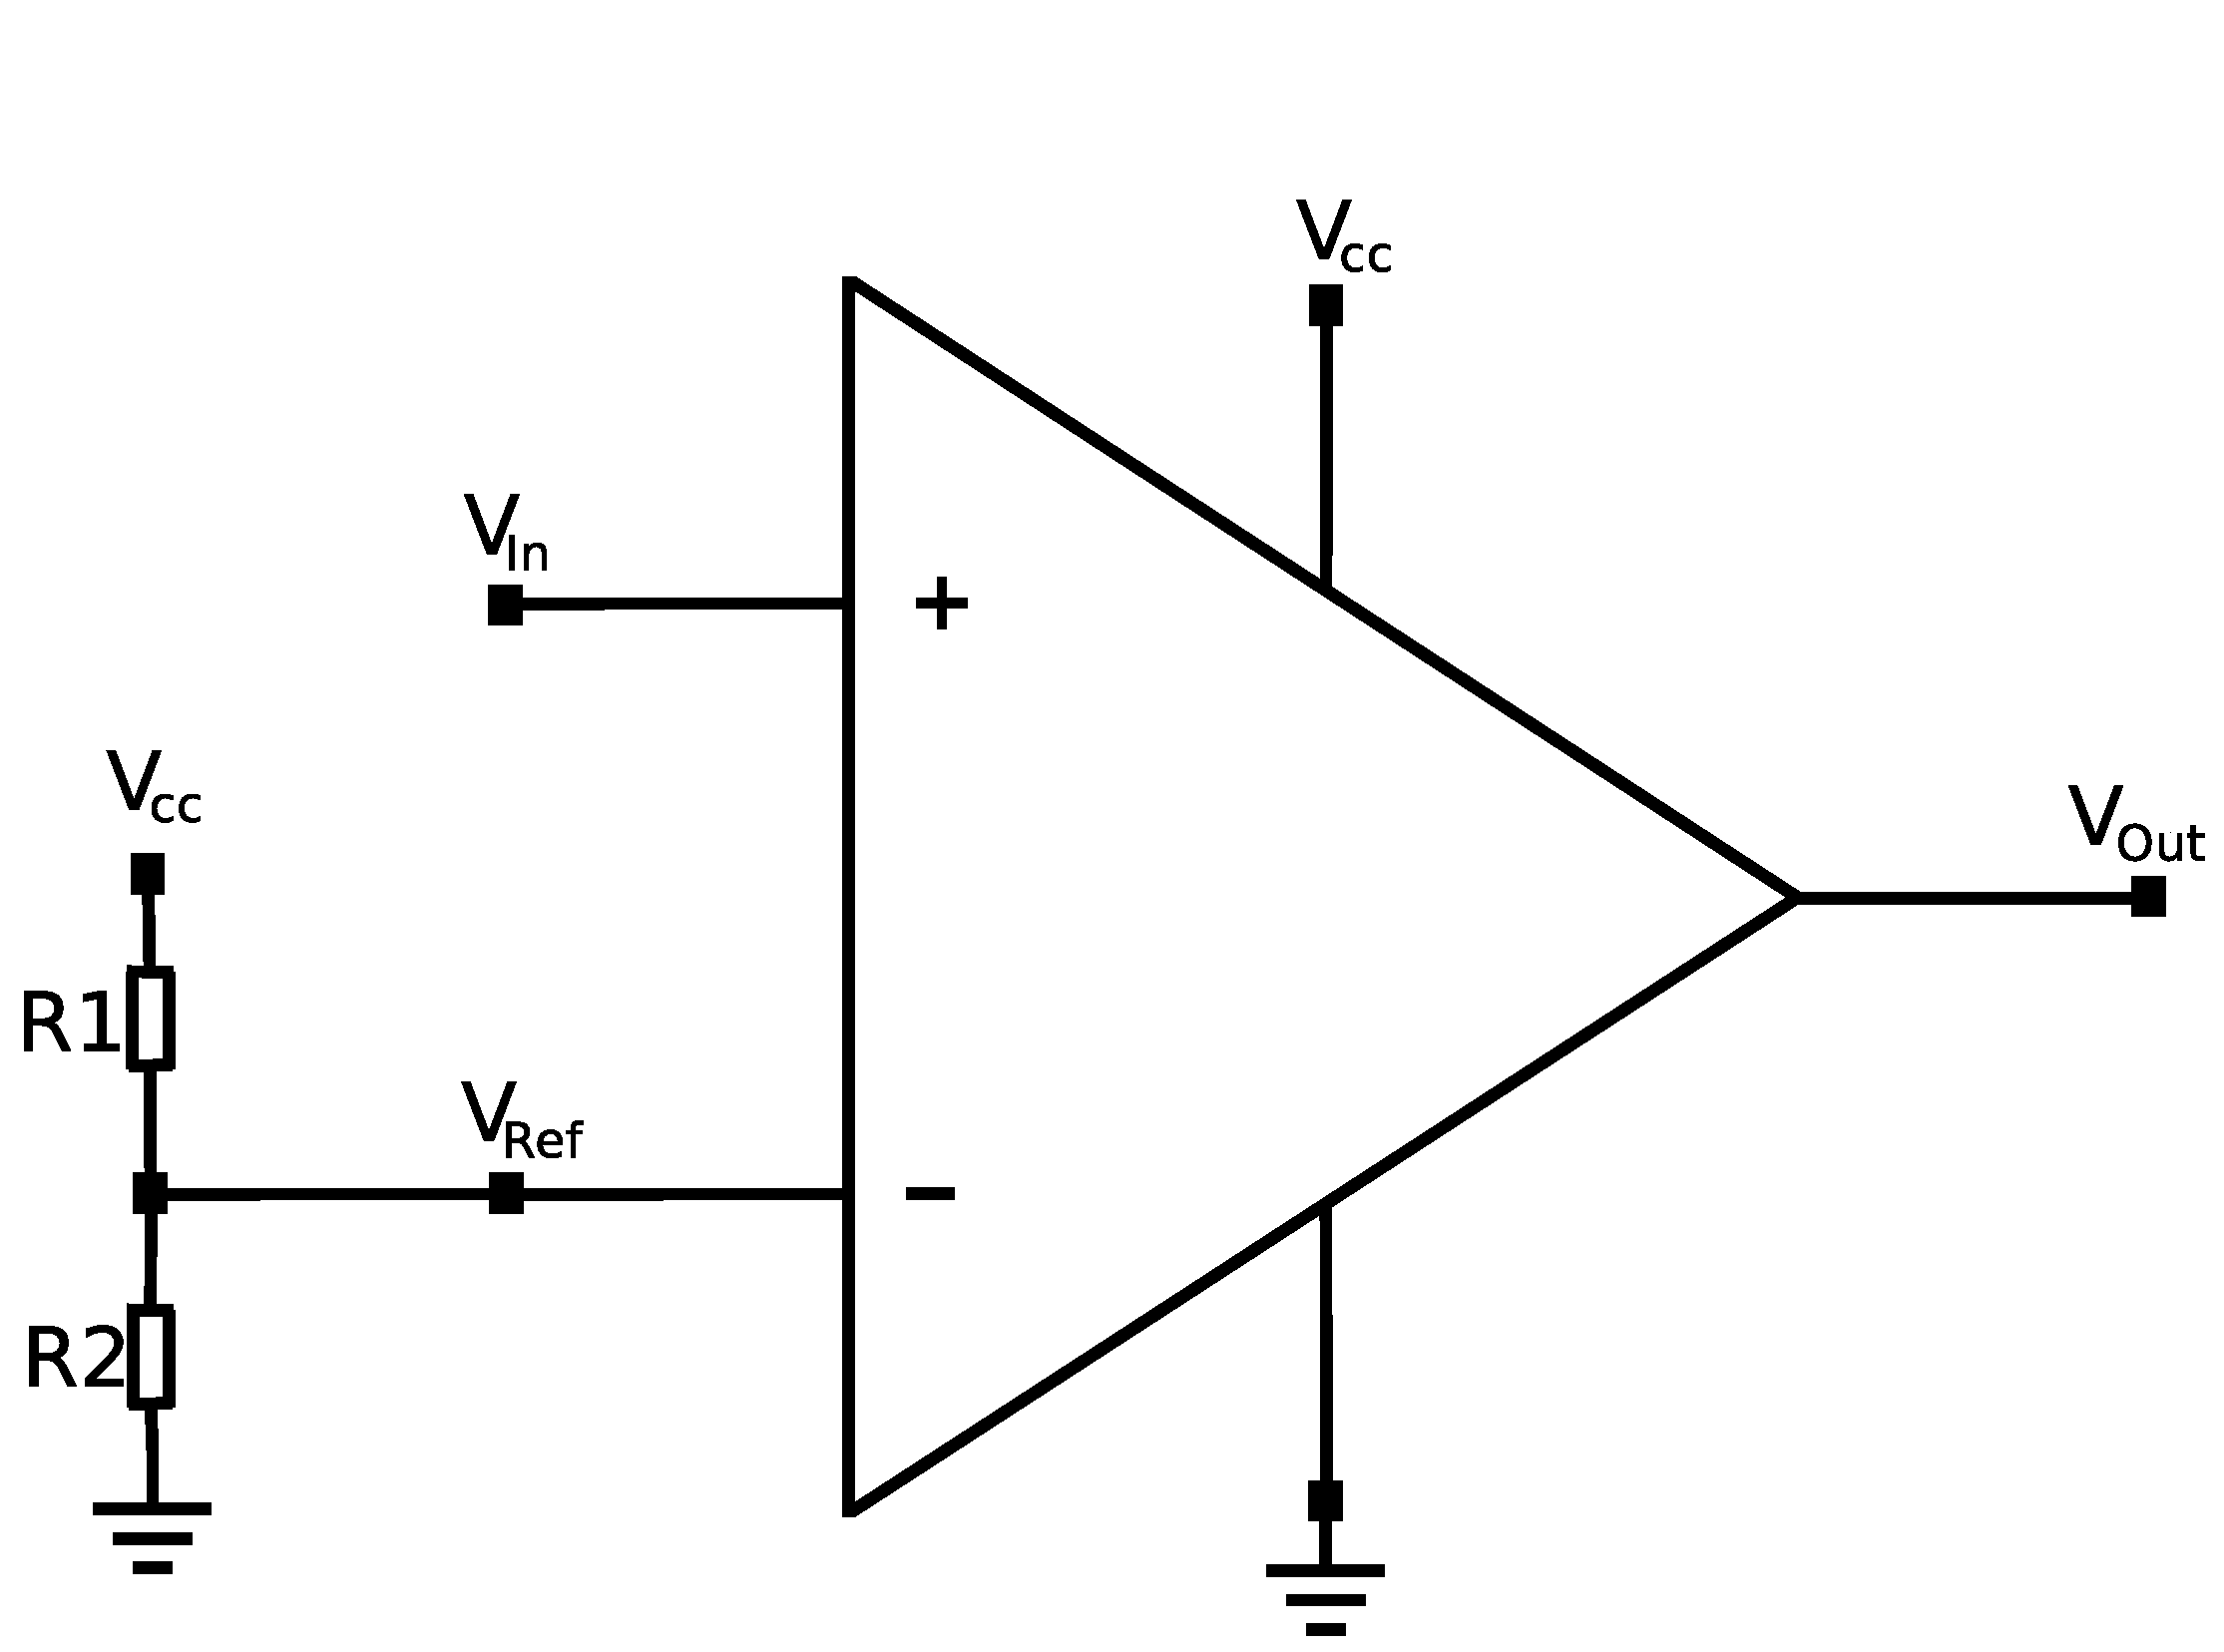
\includegraphics[width=0.6\linewidth]{fig/nao_inversor}
	\caption{Circuito comparador não inversor.}
	\label{fig:comparador1}
	\end{minipage}
\end{figure}

A Figura~\ref{fig:comparador1} mostra um comparador de tensão utilizando a
configuração não inversora. Nessa configuração de comparação é utilizado uma
tensão fixa como referência ($V_{Ref}$) na entrada inversora. A
Figura~\ref{fig:sinal1} mostra o comportamento dos sinais utilizando essa
configuração.

\begin{figure}[!h]
	\centering
	\begin{minipage}[c]{\textwidth}
	\centering
	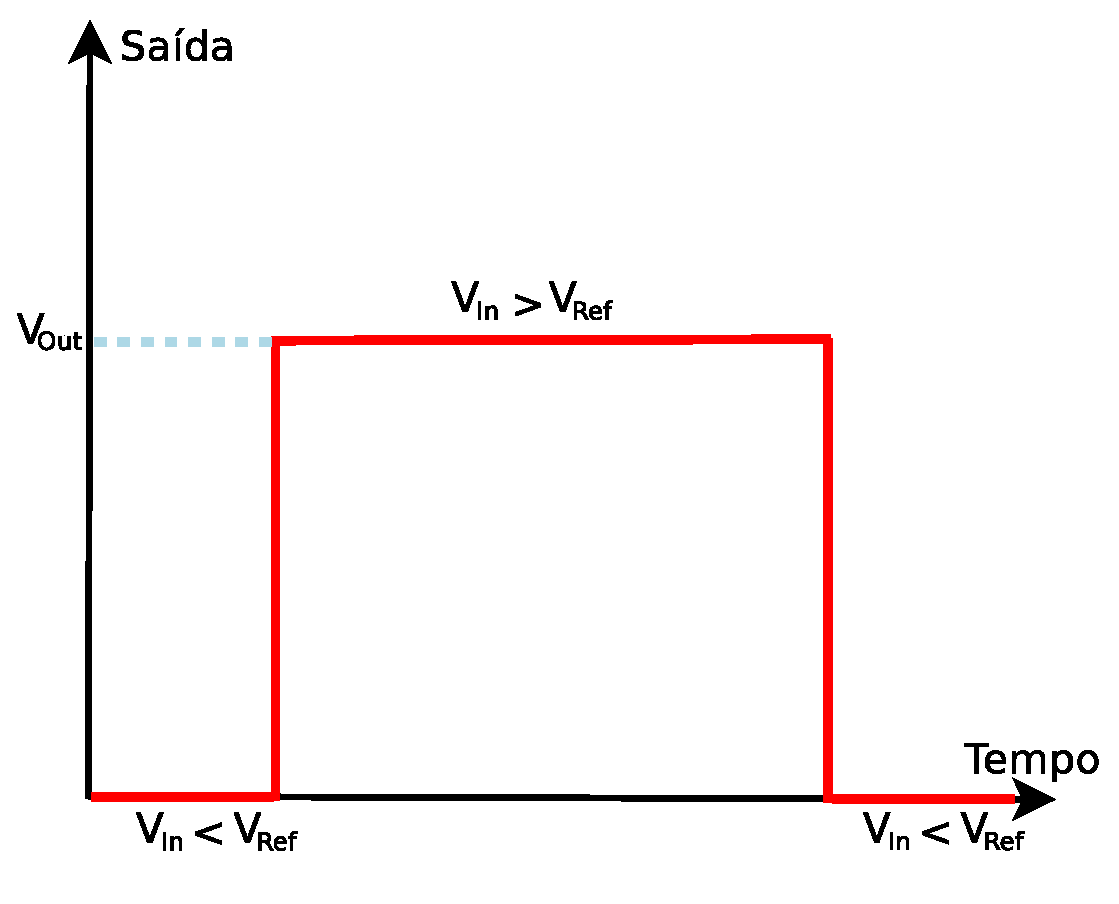
\includegraphics[width=0.5\linewidth]{fig/comparador_nao_inversor}
	\caption{Comportamento do sinal de saída do comparador não inversor.}
	\label{fig:sinal1}
	\end{minipage}
\end{figure}

Enquanto a tensão de referência for maior que o sinal da entrada não inversora
($V_{In}$), a saída tende para 0~V. Contudo, quando a tensão da entrada não
inversora é maior que a tensão de referência, a saída ($V_{Out}$) tende para a
magnitude da tensão utilizada como alimentação do amplificador operacional
($V_{cc}$). Por
exemplo, se o amplificador for alimentado com 15~V a saída desse componente se
aproximaria de 15~V, porém nunca seria 15~V. Idealmente, o valor de saída nesse
caso tenderia para o infinito, contudo na prática isso não acontece devido a
diversos fatores físicos do componente.

\begin{figure}[!h]
	\centering
	\begin{minipage}[c]{\textwidth}
	\centering
	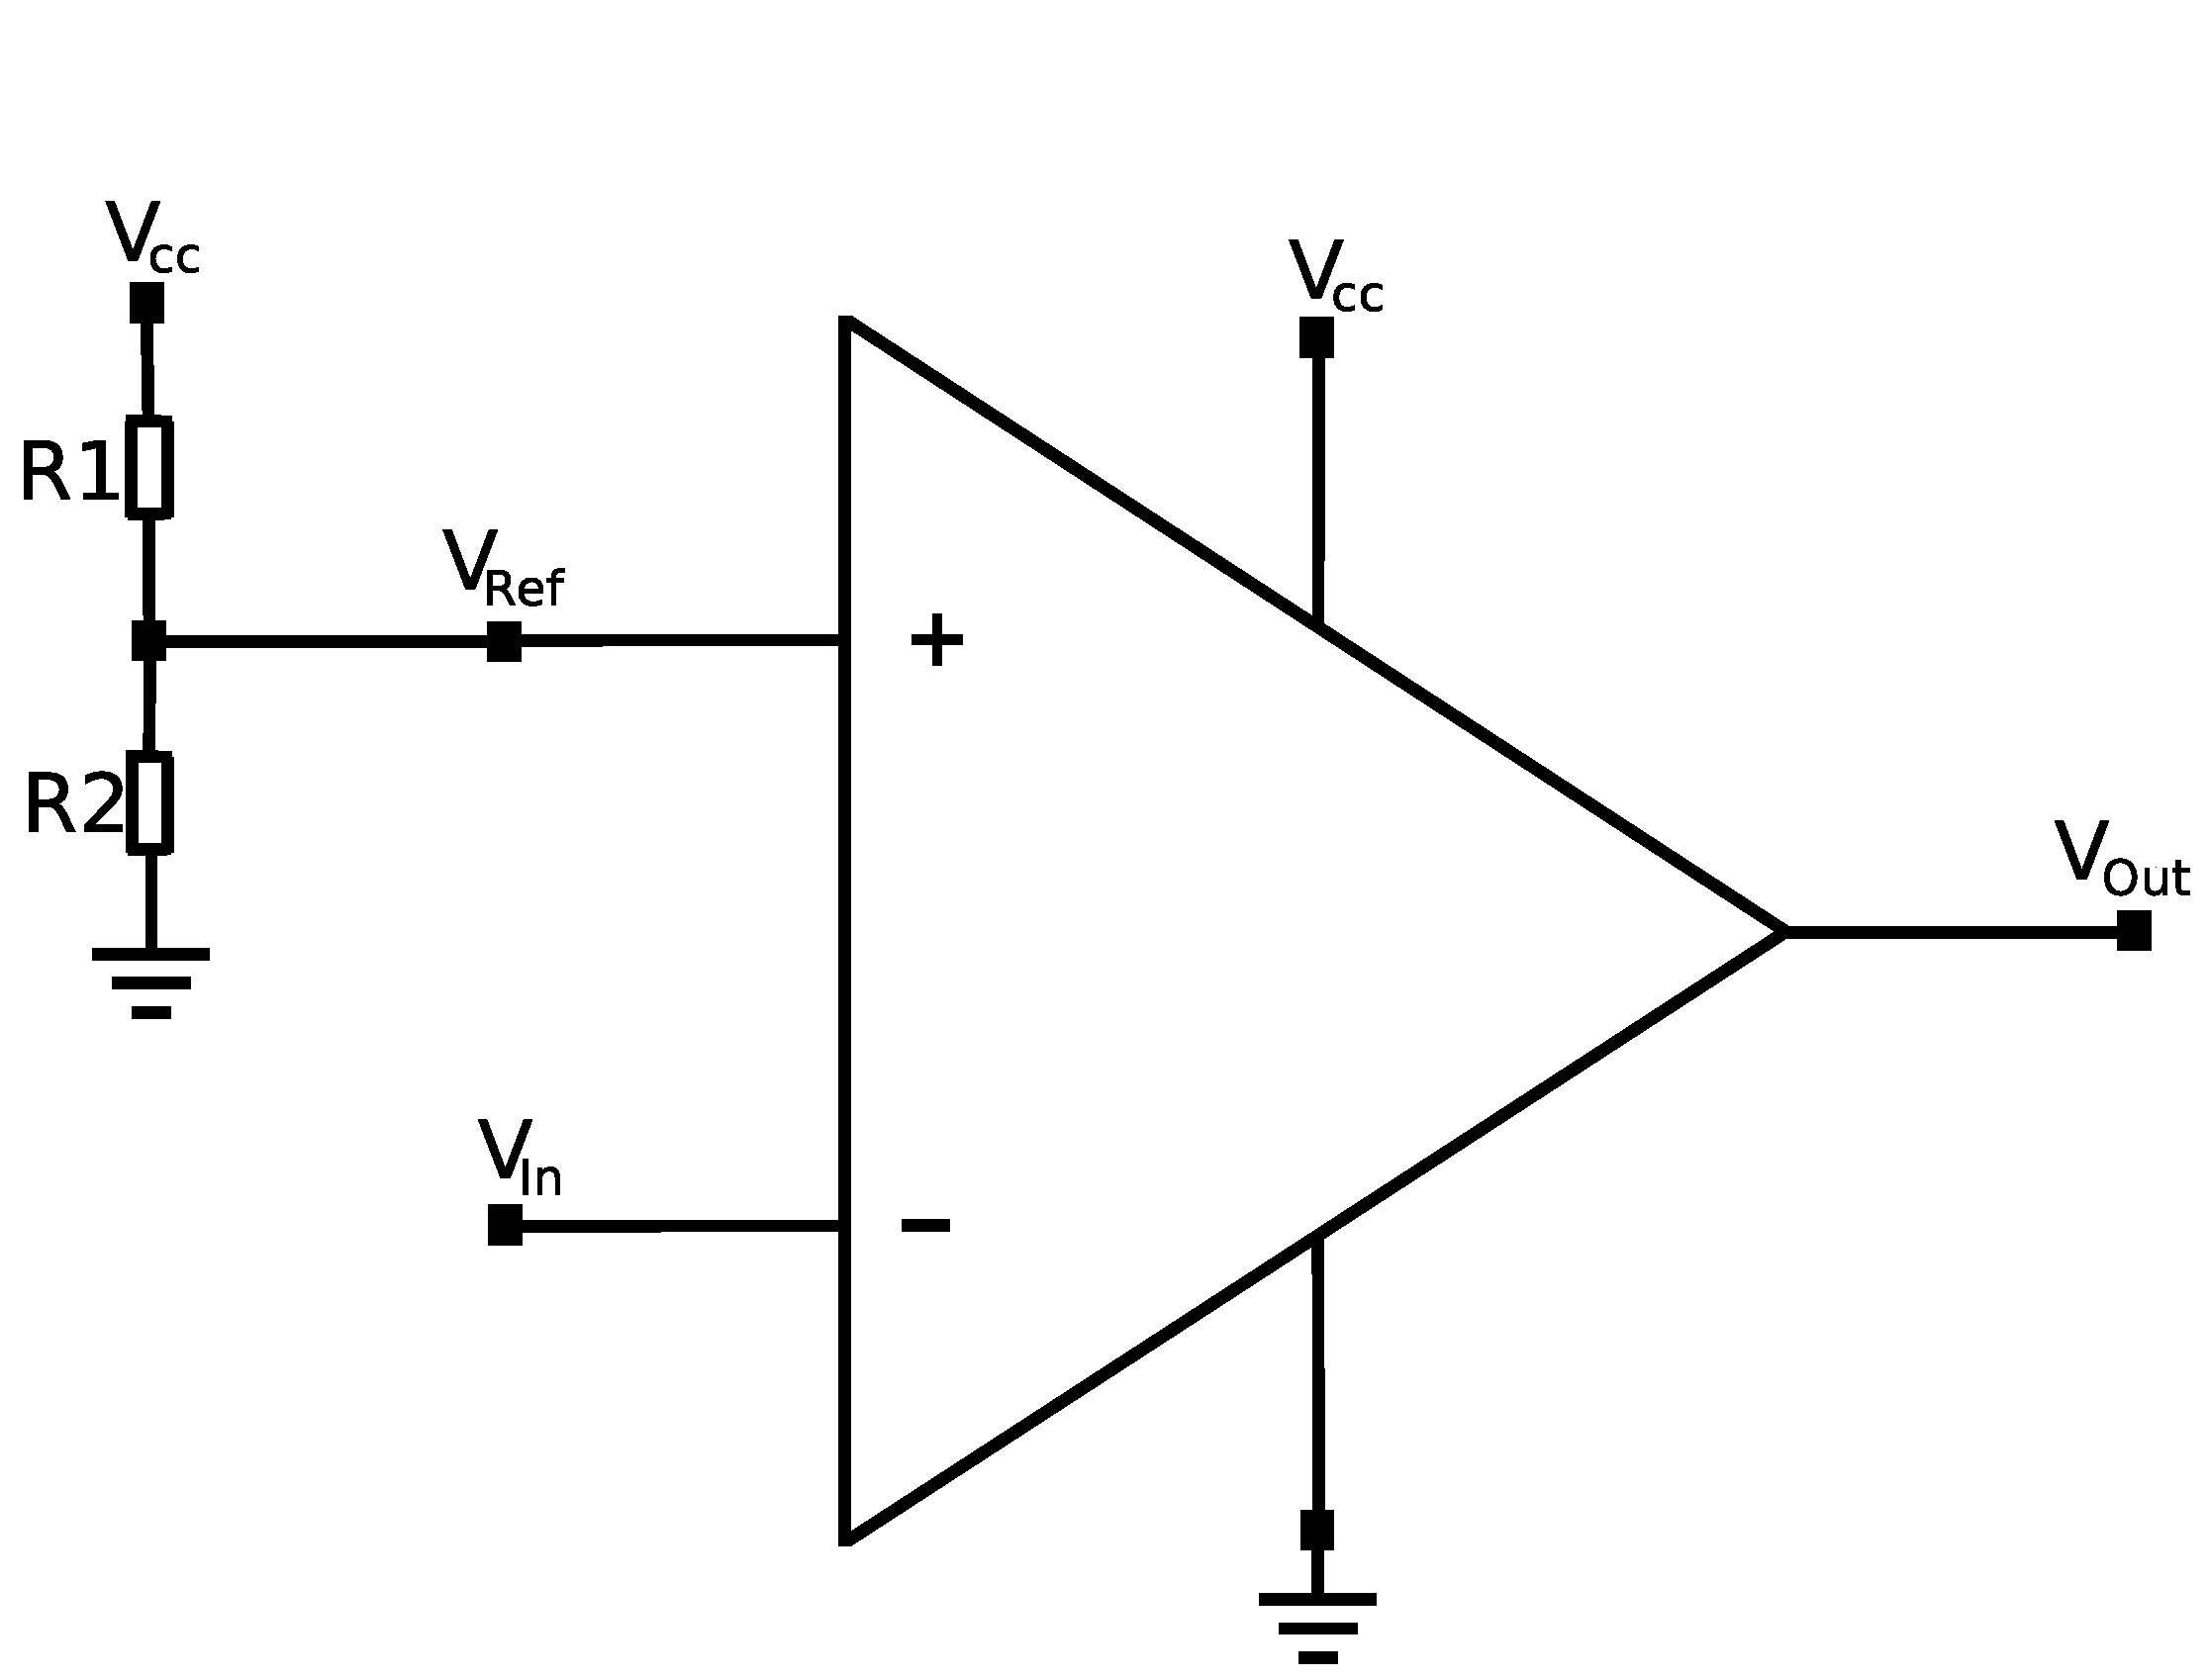
\includegraphics[width=0.5\linewidth]{fig/inversor}
	\caption{Circuito comparador não inversor.}
	\label{fig:comparador2}
	\end{minipage}
\end{figure}

Já a Figura~\ref{fig:comparador2} mostra um comparador de tensão utilizando a
configuração inversoa. Nessa configuração também é utilizado uma tensão de
refêrencia, porém é colocada na entrada não inversora.O comportamento dos sinais
utilizando a configuração inversora é mostrado na Figura~\ref{fig:sinal2}. 


\begin{figure}[!h]
	\centering
	\begin{minipage}[c]{\textwidth}
	\centering
	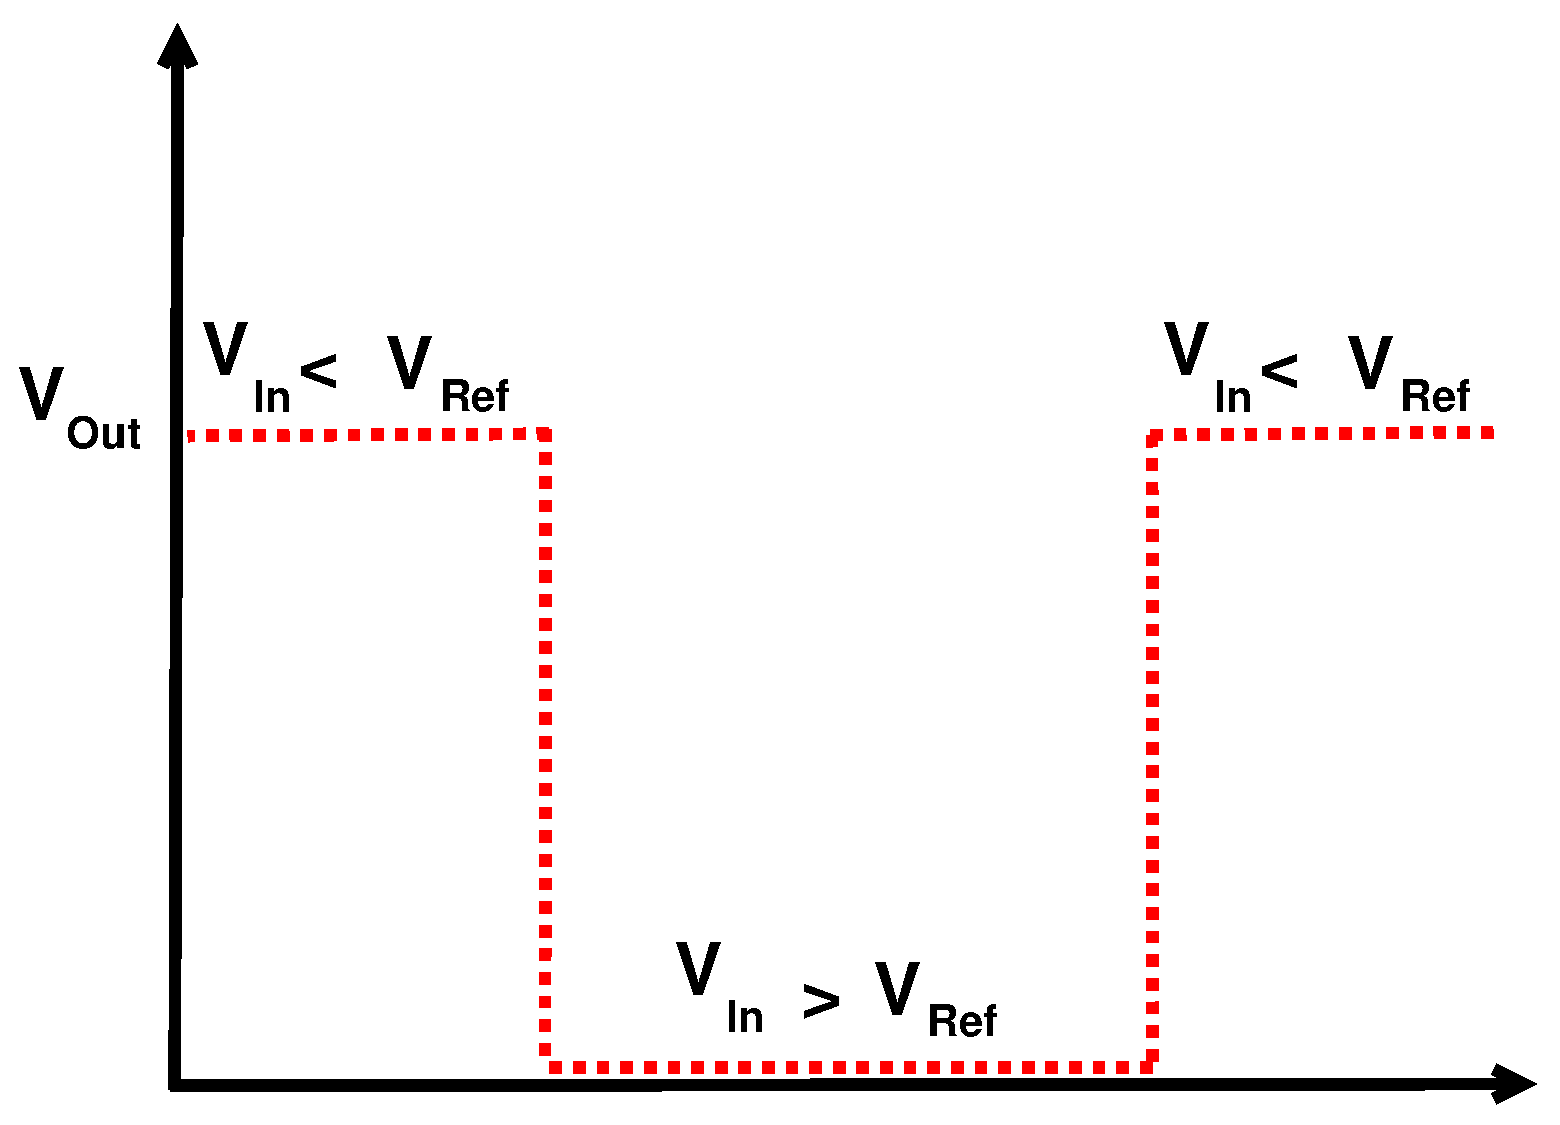
\includegraphics[width=0.5\linewidth]{fig/comparador_inversor}
	\caption{Comportamento do sinal de saída do comparador inversor.}
	\label{fig:sinal2}
	\end{minipage}
\end{figure}

A configuração de comporador inversor ocorre, como o próprio nome sugere, um
comportamento oposto ao comparador não inversor. Enquanto a tensão de refência é
maior que a tensão da entrada não a saída tende para a magnitude da tensão de
alimentação do operador operacional. Já quando ocorre o contrário,  a tensão da
saída tende para 0~V.

\end{section}


\begin{section}{Conectores de Áudio}

Sinais de áudio podem ser transmitidos através de vários tipos de conectores.
Por exemplo, é possivel reproduzir os sinais de áudio produzidos por uma
guitarra para uma caixa acústica amplificada. Geralmente utiliza-se o conector
P10 para realizar a transmissão da guitarra para a caixa acústica. Já para fones
de ouvidos, por exemplo, é utilizado o conector P2. Segundo uma matéria
disponível na BBC News~\cite{BBC}, o conector P2 é utilizado desde o século XIX.
Os conectores mais utilizados são os conectores TS e TRS que serão brevemente
descritos a seguir.

\begin{subsection}{Conector TS}

O TS é um conector utilizado para transmitir sinais analógicos e são mais
utilizados natransmissão de áudio. Há diversos tamanhos de conectores TS e são
comercializados com diferentes diâmetros, como 2.5~mm, 3.5~mm e 6.35~mm. A
Figura~\ref{fig:TS} mostra a ilustração de um conector TS.

\begin{figure}[!h]
	\centering
	\begin{minipage}[c]{\textwidth}
	\centering
	\includegraphics[width=0.9\linewidth]{fig/ts}
	\caption{Conector TS.}
	\label{fig:TS}
	\end{minipage}
\end{figure} 

O conector TS possui somente um canal de transmissão de sinal analógico é
um conector mono~\cite{ts}. O TS possui dois pinos que são separados entre si por
um anel isolante. O pino Tip que  fica localizado no final do conector é 
utilizado para realizar a  transmissão do sinal. Já o pino Sleeve é responsável
por ser a referência (GND) do conector.

\end{subsection}

\begin{subsection}{Conector TRS}
O TRS também é um conector utilizado para transmissão de sinais analógicos. Esse
conector é normalmente chamado de P3, por possuir três pinos, porém este nome
está tecnicamente incorreto pois a nomenclatura é denominada de acordo com o
diâmetro de cada conector. Sendo assim a nomenclatura P2, por exemplo, podendo
ser tanto TS quanto TRS,  refere-se a conectores com diâmetro de 3.5~mm, assim
como P10 refere-se a conectores de 6.35~mm. A Figura~\ref{fig:TRS} mostra a
ilustração de um conector TRS.

\begin{figure}[!h]
	\centering
	\begin{minipage}[c]{\textwidth}
	\centering
	\includegraphics[width=0.9\linewidth]{fig/trs}
	\caption{Conector TRS.}
	\label{fig:TRS}
	\end{minipage}
\end{figure} 

O conector TRS possui três pinos que, assim como o TS, também são separados 
entres sim por anéis isolantes. Contudo, o TRS pode transmitir dois sinais
analógicos simultâneamente, sendo, portanto, um conector estéreo. O pino Sleeve,
ou GND, é a referênca do conector. O pino Ring, também chamado de Right ( canal 
direito da transmissão ) é o  pino central do conector. Já Tip, pino localizado
no final do conector, também é conhecido por Left, pois é responsável por
transmitir um sinal pelo canal esquerdo.

É possível transformar um conector TRS em TS, ou seja, transformar um conector
estéreo em mono. Para isso é necessário realizar um curto circuito entre os
pinos Ring e Tip do conector estéreo. Quando um sinal é enviado para o Ring e
Tip, como eles estão curto circuitados, os dois canais transmitem o mesmo
sinal em somente um canal. Sendo assim, o conector TRS age como se fosse um
conector TS. Esse tipo de alteração é necessária caso o dispositivo que receba a
entrada do conector seja mono e o conector seja TRS. 

\end{subsection}

\end{section}


\begin{section}{Kicad}
Para o desenvolvimento de placas de circuito impresso, é primeiramente projetar
o \textit{layout} do circuito. Para realizar essa tarefa é necessário a
utilização de um \textit{software} EDA (do inglês, \textit{electronic design
automation}). Existem vários \textit{software} EDA, como o Eagle~\cite{eagle}. O
Eagle é um \textit{software} amplamente utilizado para o desenvolvimento de
placas de circuito impresso, contudo possui a desvantagem de não ser um
\textit{software} livre que é liberado gratuitamente apenas para uso pessoal e
não comercial. Além disso, a versão gratuita não possui uma quantidade limitada
de ferramentas de desenvolvimento. Para ter acesso a essas ferramentas é
necessário adquidir uma assinatura que pode ser mensal ou anual. Os preços dessa
assinatura variam de R\$~52.91 a R\$~3227.40~\cite{EagleAssinatura}

Existem de ferramentas EDA que são de código aberto e gratuitos. O
Kicad~\cite{kicad} é o  \textit{software} de código aberto e gratuito mais
utilizado entre os desenvolvedores. Essa ferramenta oferece recursos necessário
para o desenvolvimento de quase todo tipo de projeto. Obviamente que não
há disponível todas as bibliotecas de componentes possíveis. Po exemplo, não há
uma biblioteca para o componente PJ324~\cite{pj324}. Contudo, há a possibilidade
de desenvolvimento de bibliotecas próprias e disponibilizá-las em repositórios,
como o Github~\cite{github}, para que qualquer pessoa possa utilizá-la em
projetos pessoais.  
\end{section}



\begin{section}{Captura de Áudio}

Para o desenvolvimento de uma aplicação de captura ou reprodução de áudio é
necessário a utilização de alguma API. Uma API (do inglês, \textit{application
programing interface}) é uma interface que define o contrato para que duas
aplicações se comuniquem entre si~\cite{API17}. A utilização de uma API pode
simplificar o desenvolvimento de aplicações, contudo há algumas limitações, como
linguagem e plataforma utilizada. 

Existem várias API para o desenvolvimento de aplicações de áudio. Agumas APIs são
nativas do sistema operacional, portanto cada sistema operacional possui APIs
específicas. A grande desvantagem de utilizar APIs nativas de um determinado
sistema operacional é que, para a utilização da mesma aplicação em outro sistema
operacional, é necessario a reescrita do códígo utilizando um API suportada pelo
sistema operacional onde deseja-se executar a aplicação. 

A camada de áudio de sistemas operacionais baseados em Linux, por
exemplo, possui o ALSA~\cite{alsa} e também o OSS~\cite{oss} como
\textit{drivers} que permitem a manipulação de áudios e cada um driver possui
uma API para o desenvolvimento de aplicações. A camada de áudio do windows
também ferramentas próprias de manipulação de áudio. Uma alternativa para ajuda
na portabibilidade da aplicação de áudio desenvolvida é utilizar APIs
multiplataformas.

Uma ferramenta bastante utilizada para o desenvolvimento de aplicações de áudio
é o PortAudio~\cite{portaudio}, uma biblioteca de código aberto,
multiplataforma, que permite escrever programas em C/C++ para realizar gravação
e reprodução de áudios. A Figura~\ref{fig:portaudio} mostra a arquitetura do
PortAudio.

\begin{figure}[!h]
	\centering
	\begin{minipage}[c]{\textwidth}
	\centering
	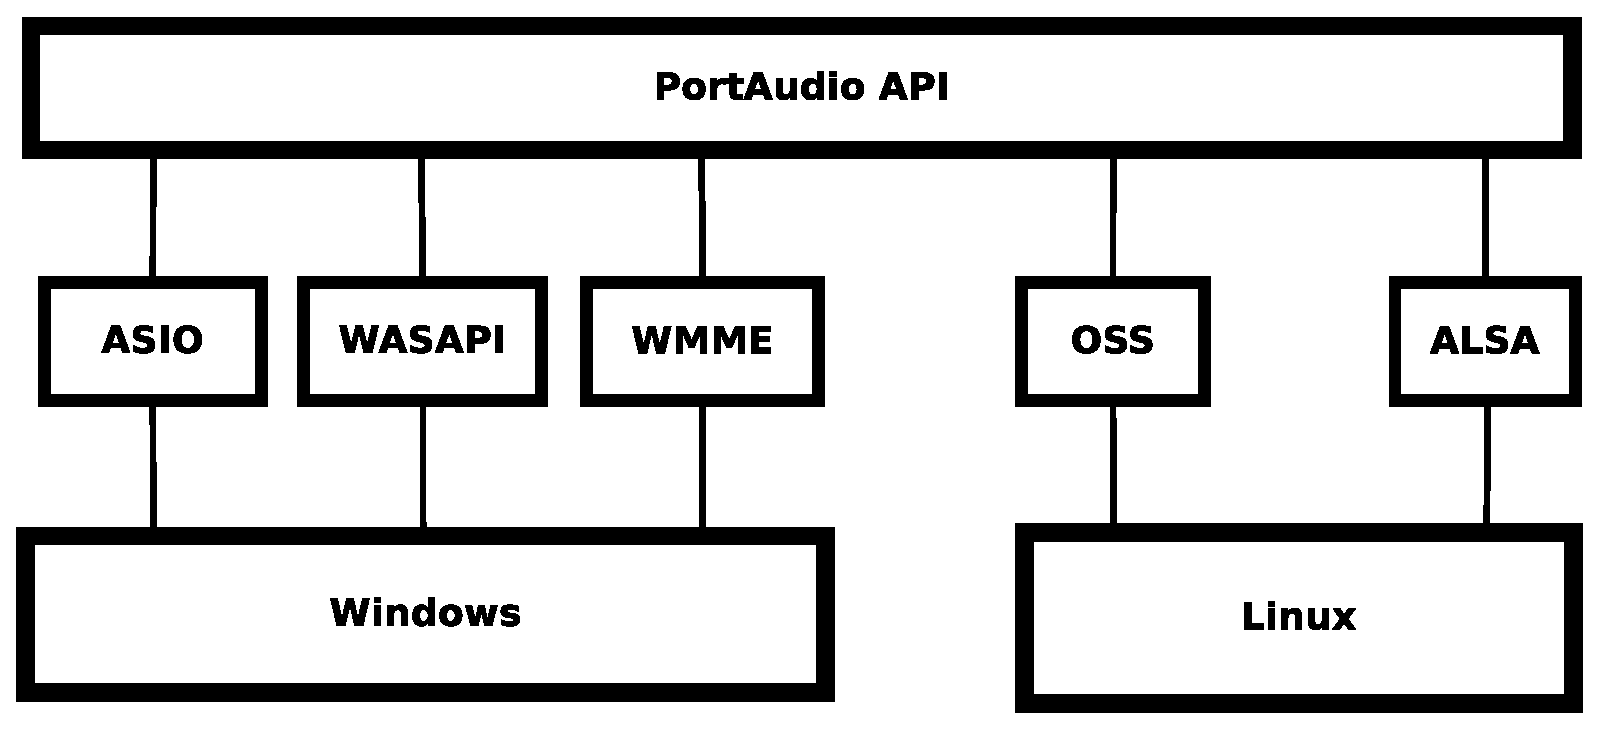
\includegraphics[width=0.7\linewidth]{fig/portaudio}
	\caption{Arquitetura do PortAudio.}
	\label{fig:portaudio}
	\end{minipage}
\end{figure} 

O PortAudio possui suporte para maioria das APIs nativas de cada sistema
operacional. É realizado uma comunicação entre o PortAudio e as APIs nativas. A
grande vantagem de utilizar essa ferramenta é que não é necessário aprender cada
API nativa dos sistemas operacionais. Dessa forma é possível utilizar o mesmo
código em diferentes sistemas operacionais, facilitando a portabilidade do
\textit{software} desenvolvido.

A desvantagem de utilizar o PortAudio é que essa ferramenta não fornece total
suporte para as funcionalidades de cada API nativa. Por exemplo, o PorAudio não
fornece conversão de taxa de amostragem se for solicitado uma taxa de amostragem
que não seja suportada pela API de áudio nativa. Outro bom exemplo é que o ASIO
SDK permite apenas que uma aplicação seja executada por vez, dessa forma o
PortAudio, atualmente, não suporta a execução de várias aplicações
simultaneamente.

\end{section}

\begin{section}{X11 e Xlib}

O X Window System, X ou X11, é um sistema de janelas criados pela MIT (do
inglês, \textit{Massachusetts Institute of Technology})~\cite{xlib}. Esse
sistema atualmente está na sua décima primeira versão --- por isso é também 
chamada de X11 --- que foi publicada em 1987. O X11 é um protocolo que funciona
no modelo cliente-servidor e é utilizado como padrão para GUIs (do inglês,
\textit{graphical user interface}) em sistemas baseados em UNIX e Linux. Uma
visão geral da arquitetura do X Window System é mostrado na
FIgura~\ref{fig:x11}.

\begin{figure}[!h]
	\centering
	\begin{minipage}[c]{\textwidth}
	\centering
	\includegraphics[width=0.7\linewidth]{fig/X11}
	\caption{Arquitetura do modelo cliente-servidor do X11.}
	\label{fig:x11}
	\end{minipage}
\end{figure} 

O servidor C é executado em computadores com telas de bitmap. O servidor
distribui a entrada do usuário e aceita pedidos de saída de vários programas
cliente através de uma variedade de diferentes canais de comunicação entre
processos~\cite{suse}. É possível criar diversas aplicações utilizando o X11,
como criação de interfaces gráficas para usuários e execução dos movimentos e
eventes de clique do \textit{mouse}. 

As aplicações funcionam como cliente e são desenvolvidas utilizando a
Xlib~\cite{xlib}, uma biblioteca cliente do protocolo X escrita em C. A Xlib
realiza o intermédio entre o cliente (aplicação) e o servidor X.  
\end{section}

\end{chapter}
